\chapter{Perancangan}
\label{chap:perancangan}

Pada bab ini akan dijelaskan perancangan mengenai simulator yang akan dibangun untuk pertumbuhan wirausaha. Perancangan yang dibuat akan meliputi diagram kelas beserta penjelasannya dan rancangan antarmuka dari perangkat lunak.


\section{Diagram Kelas}
\label{sec:perancangankelas}

Dalam membuat simulator diperlukan sebuah GUI atau Interface untuk bisa menggambarkan kinerja suatu sistem. Berdasarkan hasil pengembangan diagram kelas pada bab analisis \ref{fig:CD1}, dibuatlah diagram kelas rinci untuk memenuhi kebutuhan dalam membangun simulator. Deskripsi kelas beserta fungsinya akan dijelaskan pada subbab selanjutnya.

\begin{figure} [H]
	\centering  
	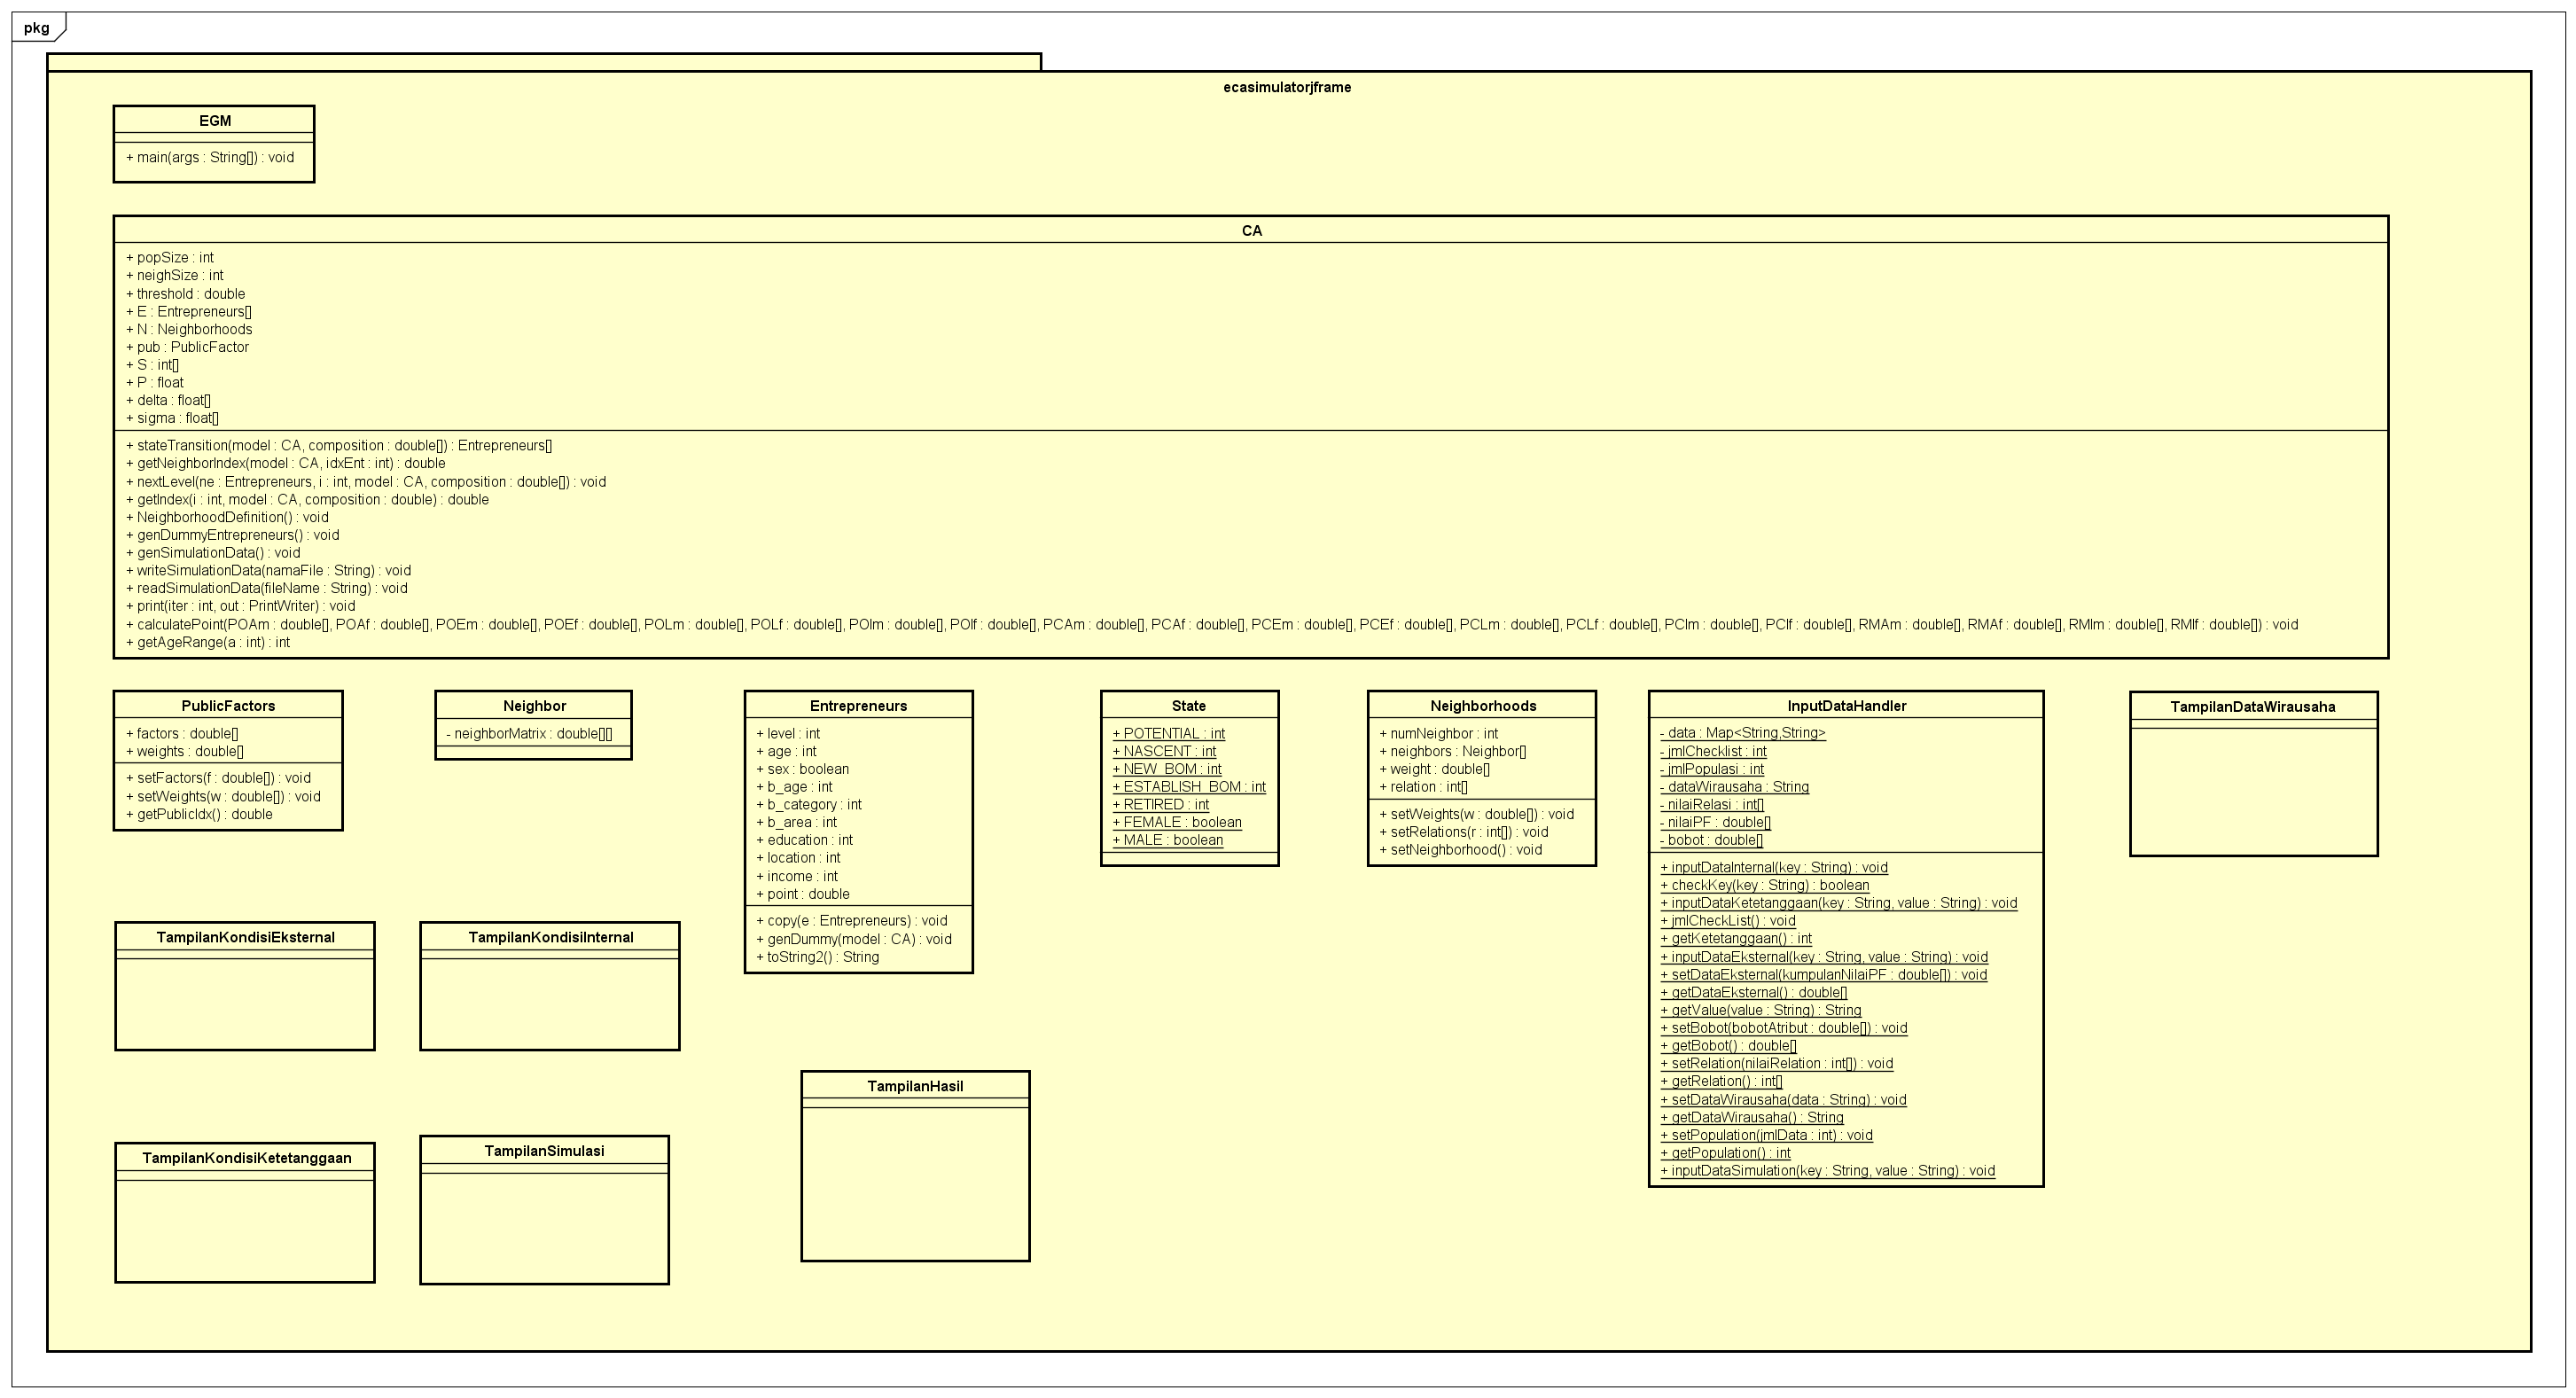
\includegraphics[width=18cm, height=12cm]{ClassDiagram3} 
	\label{fig:classdiagram2} 
\end{figure}


\subsection{Kelas TampilanKondisiInternal}
Kelas ini merupakan kelas untuk menampilkan seluruh atribut umum dari seorang wirausaha yang dapat dipilih menggunakan \textit{checkbox}, atribut yang dipilih nantinya akan mempengaruhi ketetanggaan antara wirausaha yang satu dengan wirausaha lainnya. Setelah itu, \textit{user} diminta mengisi bobot untuk masing-masing atribut yang sudah dichecklist melalui \textit{textfield}.

\subsection{Kelas TampilanKondisiKetetanggaan}
Kelas ini merupakan kelas untuk menampilkan atribut yang sudah dipilih dari kelas TampilanKondisiInternal. \textit{User} dapat memilih atribut mana saja yang akan ditetapkan menjadi kondisi ketetanggaan untuk satu wirausaha ke wirausaha lainnya. Selain itu, \textit{user} diminta untuk mengisi hubungan ketetanggaan khusus untuk 4 atribut yaitu umur, level, pendapatan dan pendidikan jika \textit{user} men-checklist salah satu atau bahkan keempat-empatnya dari atribut tersebut. Untuk atribut jenis kelamin, lokasi usaha dan bidang usaha tidak dapat ditetapkan menjadi 3 jenis karena jenisnya hanya satu yaitu sama dengan. Alasan ketiga atribut tersebut tidak bisa ditetapkan menjadi 3 jenis karena ketiga atribut tersebut tidak bisa diurutkan atau dibandingkan seperti atribut a lebih besar dari atribut b.

\subsection{Kelas TampilanKondisiEksternal}
Kelas ini merupakan kelas untuk menampilkan faktor eksternal yang mempengaruhi pertumbuhan wirausaha. Dalam kasus ini ditetapkan 4 faktor saja yaitu program pemerintah, dinamika pasar, norma,sosial dan budaya, serta infrastruktur fisik dan akses layanan. \textit{User} diminta untuk mengisi bobot untuk setiap faktor dan total dari semua bobot harus 100\%.

\subsection{Kelas DataWirausaha}
Kelas ini merupakan kelas untuk membuka file data wirausaha yang akan disimulasikan, lalu menampilkannya ke tabel. Isi datanya berupa :
\begin{enumerate}
	\item Jenis Kelamin
	
	
	Tipe data boolean, true untuk pria dan false untuk wanita
	\item Umur
	
	
	Tipe data integer (dalam tahun)
	\item Usia Bisnis
	
	
	Tipe data integer, usia dalam bulan.
	\item Kategori Usaha
	
	
	Tipe data integer, masing-masing angka mendeskripsikan kategori usaha yang berbeda, yaitu :
		\begin{enumerate}
		\item 0 untuk makanan
		\item 1 untuk minuman 
		\item 2 untuk tas
		\item 3 untuk pakaian
		\end{enumerate}
	\item Subkategori
	
	
	Tipe data integer, masing-masing angka mendeskripsikan subkategori yang berbeda, yaitu :
	\begin{enumerate}
		\item 0 untuk makanan ringan
		\item 1 untuk makanan berat
		\item 2 untuk minuman sachet
		\item 3 untuk tas wanita
	\end{enumerate}
		
		\item Pendidikan
		
		
		Tipe data integer, masing-masing angka mendeskripsikan tingkat pendidikan yang berbeda, yaitu :
		\begin{enumerate}
			\item 0 untuk tingkat pendidikan rendah
			\item 1 untuk sekolah dasar
			\item 2 untuk sekolah menengah pertama
			\item 3 untuk sekolah menengah keatas
			\item 4 untuk sarjana (S1)
			\item 5 untuk diploma (S2)
			\item 6 untuk profesor (S3)
		\end{enumerate}
		\item Lokasi
		
		
		Tipe data integer, masing-masing angka mendeskripsikan lokasi yang berbeda, yaitu :
		\begin{enumerate}
			\item 0 untuk Banda Aceh
			\item 1 untuk Medan
			\item 2 untuk Padang
			\item 3 untuk Pekanbaru
			\item 4 untuk Palembang
			\item 5 untuk Bandar Lampung
			\item 6 untuk Serang
			\item 7 untuk Jakarta
			\item 8 untuk Bandung
			\item 9 untuk Semarang dan Surakarta
			\item 10 untuk Surabaya
			\item 11 untuk Denpasar
			\item 12 untuk Mataram
			\item 13 untuk Kupang
			\item 14 untuk Pontianak
			\item 15 untuk Makassar
		\end{enumerate}
		\item Pendapatan
		
		
		Tipe data integer, masing-masing angka mendeskripsikan tingkat pendapatan yang berbeda, yaitu :
		\begin{enumerate}
			\item 0 untuk pendapatan dibawah 3 juta rupiah
			\item 1 untuk pendapatan 3 juta rupiah sampai 5 juta rupiah
			\item 2 untuk pendapatan 5 juta rupiah sampai 7 juta rupiah
			\item 3 untuk pendapatan 7 juta rupiah sampai 9 juta rupiah
			\item 4 untuk pendapatan 9 juta rupiah sampai 11 juta rupiah
			\item 5 untuk pendapatan 11 juta rupiah sampai 13 juta rupiah
			\item 6 untuk pendapatan 13 juta rupiah sampai 15 juta rupiah
			\item 7 untuk pendapatan diatas 15 juta rupiah
		\end{enumerate}
		\item Level
		
		
		Tipe data integer, masing-masing angka mendeskripsikan level yang berbeda, yaitu :
		\begin{enumerate}
			\item 0 untuk level potential
			\item 1 untuk level nascent
			\item 2 untuk level new business manager
			\item 3 untuk level established 
			\item 4 untuk level retired
		\end{enumerate}
		\item Point
		
		
		Point merupakan nilai dari kondisi internal individu wirausaha. Point mempunyai tipe data double.
\end{enumerate}

\subsection{Kelas TampilanSimulasi}
Kelas ini untuk mengisi nilai a, b, c, threshold dan periode. Nilai a,b,c dan threshold bertipe double, sedangkan periode bertipe integer. Periode ini dihitung dalam bulan. Kelas ini juga untuk menghitung Continuity Index yang hasilnya akan dikirim ke kelas TampilanHasil.
\subsection{Kelas TampilanHasil}
Kelas ini untuk menampilkan hasil iterasi wirausaha untuk setiap periode (bulan).
\subsection{Kelas InputDataHandler}
Kelas ini merupakan kelas untuk mengambil dan menyimpan data masukan dari \textit{user} yang nantinya akan dipakai untuk menghitung Continuity Index.


\section{Rancangan Antarmuka}
\label{sec:rancanganantarmuka}

\subsection{TampilanKondisiInternal}

